\section*{ÔN TẬP KIỂM TRA CUỐI KÌ 1 - ĐỀ 01}
\setcounter{ex}{0}\setcounter{bt}{0}
\noindent{\bf\fontfamily{qag}\selectfont\color{violet}A. PHẦN TRẮC NGHIỆM}
\Opensolutionfile{ans}[ans/ansBTTeX1]

\begin{ex}%[Lê Quốc Dũng-Dự Án TEX TLDH5]%[0D1Y2-2]
Khẳng định nào sau đây là \textbf{đúng}?
\choice
{\True $\mathbb{N}\subset \mathbb{Z}$}
{$\mathbb{Q}\subset \mathbb{N}$}
{$\mathbb{R}\subset \mathbb{Q}$}
{$\mathbb{R}\subset \mathbb{Z}$}
\loigiai{
Chọn $\mathbb{N}\subset \mathbb{Z}$ vì mọi số tự nhiên đều là số nguyên.}
\end{ex}

\begin{ex}%[0D4B4-1]
Điểm nào sau đây thuộc miền nghiệm của bất phương trình $x+y-2>0$?
\choice
{\True $(2;1)$}
{$(0;0)$ }
{$(1;0)$ }
{$(0;1)$ }
\loigiai{
\immini{
Tập hợp các điểm biểu diễn nghiệm của bất phương trình $x+y-2>0$  là nửa mặt phẳng bờ là đường thẳng $y=x+2$  và không chứa gốc tọa độ.
Từ đó ta có điểm $(2;1)$  thuộc miền nghiệm của bất phương trình.
}
{\begin{tikzpicture}[>=stealth, scale=0.7]
\draw[->,line width = 1pt] (-2.5,0)--(0,0) node[below right]{$O$}--(4,0) node[below]{$x$};
\draw[->,line width = 1pt] (0,-2.5) --(0,3.5) node[right]{$y$};
\foreach \x in {-2,-1,1,2,3}{
\draw (\x,0) node[below]{$\x$} circle (1pt);
\draw (0,\x) node[left]{$\x$} circle (1pt);
}
\draw [pattern = horizontal lines, thick, domain=-1:4.0, samples=100] plot (\x, {-(\x)+2}) node[right]{$d$};
\draw[pattern = horizontal lines,opacity=.3, line width = 1.2pt,draw=none] plot[domain=-1:4.0] (\x, {-(\x)+2})--(-2,-2)--(-2,3)--cycle;
\clip (-2.5,-2.5) rectangle (4.0,3.5);
\draw (2,1) node[right]{$M(2;1)$} circle(2pt);
\draw[dashed] (2,0)--(2,1)--(0,1);
\end{tikzpicture}
}
}
\end{ex}

\begin{ex}C%[0D3B2-4]
Nghiệm của phương trình $\sqrt{4x^2+2x+10}=3x+1$ là
\choice
{\True $x=1$}
{ $x=\dfrac{-9}{5}$}
{$\hoac{&x=\dfrac{-9}{5}\\&x=1}$}
{$x\in\varnothing$}
\loigiai{Bình phương hai vế của phương trình đã cho, ta được
\begin{eqnarray*}
4x^2+2x+10=(3x+1)^2\Rightarrow 4x^2+2x+10=9x^2+6x+1\Rightarrow -5x^2-4x+9=0\Rightarrow x=1 \ \text{hoặc} \ x=-\dfrac{9}{5}.
\end{eqnarray*}
Thay lần lượt các giá trị trên vào phương trình đã cho, ta thấy $x=1$ thỏa mãn.\\
Vậy nghiệm của phương trình đã cho là $x=1$.
}
\end{ex}

\begin{ex}%[0D4B5-2]
Cho các mệnh đề\\
(I) Với mọi $x \in [-1;4]$ thì $-x^2+4x+5 \geq 0$.\\
(II) Với mọi $x \in (-\infty;4) \cup (5;10)$ thì $x^2+9x-10>0$. \\
(III) Với mọi $x \in [2;3]$ thì $x^2-5x+6 \leq 0$.
\choice
{\True Mệnh đề (I) và (III) đúng}
{Chỉ mệnh đề (I) đúng}
{Chỉ mệnh đề (III) đúng}
{Cả ba mệnh đề đều sai}
\loigiai{
\begin{itemize}
\item $-x^2+4x+5 \geq 0 \Leftrightarrow -1 \leq x \leq 5$, suy ra mệnh đề (I) đúng.
\item $x^2+9x-10>0 \Leftrightarrow \hoac{& x>1 \\& x<-10}$, suy ra mệnh đề (II) sai.
\item $x^2-5x+6 \leq 0 \Leftrightarrow 2 \leq x \leq 3$, suy ra mệnh đề (III) đúng.
\end{itemize}
}
\end{ex}

\begin{ex}%[0H1B1-1]
Cho tứ giác $ABCD$. Có bao nhiêu véc-tơ khác véc-tơ-không có điểm đầu và cuối là các đỉnh của tứ giác?
\choice
{$4$}
{$6$}
{$8$}
{\True $12$}
\loigiai{
Xét các véc-tơ có điểm $A$ là điểm đầu thì có các véc-tơ thỏa mãn bài toán là $\overrightarrow{AB}, \overrightarrow{AC}$, $ \overrightarrow{AD}$.\\
Vậy có $3$ véc-tơ.
Tương tự cho các điểm còn lại $B$, $C$, $D$.}
\end{ex}

\begin{ex}%[0D2Y3-3]
Cho hàm số bậc hai $y=a{x^2}+bx+c$ $\left(a\ne 0\right)$ có đồ thị $\left(P\right)$, đỉnh của $\left(P\right)$ được xác định bởi công thức nào?
\choice
{\True $I\left(-\dfrac{b}{2a};\dfrac{\Delta}{4a}\right)$}
{$I\left(-\dfrac{b}{a};\dfrac{\Delta}{4a}\right)$}
{$I\left(\dfrac{b}{a};\dfrac{\Delta}{4a}\right)$}
{$I\left(-\dfrac{b}{2a};\dfrac{\Delta}{2a}\right)$}
\loigiai{
Đỉnh của parabol $\left(P\right)\colon y=a{x^2}+bx+c$ $\left(a\ne 0\right)$ là điểm $I\left(-\dfrac{b}{2a};-\dfrac{\Delta}{4a}\right)$.}
\end{ex}

\begin{ex}%[0H2Y1-1]
Cho $\alpha$ là góc tù. Khẳng định nào sau đây \textbf{đúng}?
\choice
{$\sin \alpha<0$}
{$\cos \alpha>0$}
{\True $\tan \alpha<0$}
{$\cot \alpha>0$}
\loigiai{
Do $\alpha$ là góc tù nên $\sin\alpha>0$, $\cos\alpha<0$, $\tan\alpha<0$ và $\cot\alpha<0$.
}
\end{ex}

\begin{ex}%[VanLo HoaTrung, du an tex hoa tai lieu 10]%[0D4Y4-1]
Trong các cặp số sau đây, cặp nào thuộc nghiệm của bất phương trình: $x-4y+5>0$?
\choice
{$(-5;0)$}
{$(-2;1)$}
{\True $(0;0)$}
{$(1;3)$}
\loigiai{
\begin{itemize}
\item Thay tọa độ điểm $(-5;0)$ vào bất phương trình ta được $-5-4.0+5>0$ (sai);
\item Thay tọa độ điểm $(-2;1)$ vào bất phương trình ta được  $-2-4.1+5>0$ (sai);
\item Thay tọa độ điểm $(0;0)$ vào bất phương trình ta được $0-4.0+5>0$ (đúng);
\item Thay tọa độ điểm $(1;3)$ vào bất phương trình ta được $1-4.3+5>0$ (sai).
\end{itemize}
}
\end{ex}

\begin{ex}%[0D1B3-2]
\immini{Cho các tập hợp $A$, $B$, $C$ được minh họa bằng biểu đồ Ven như hình vẽ. Phần tô màu xám trong hình là biểu diễn của tập hợp nào sau đây?
\choice
{$A\cap B\cap C$}
{$(A\setminus C)\cup (A\setminus B)$}
{$(A\cup B)\setminus C$}
{\True $(A\cap B)\setminus C$}
}{\begin{tikzpicture}[smooth,font=\footnotesize,scale=0.8]
\def\miena{(0,0) to[bend left=90] (2,2) to[bend left=90] (0,0)}
\def\mienb{(1,0) to[bend left=90] (3,2) to[bend left=90] (1,0)}
\def\mienc{(0,-1) to[bend left=90] (2,1) to[bend left=90] (0,-1)}
\begin{scope}
\clip \miena;
\draw[pattern=north east lines,pattern color=orange] \mienb;
\draw[draw=none,fill=white] \mienc;
\end{scope}
\draw \miena \mienb \mienc
(0.5,1.2) node{$A$}
(2.6,0.9) node{$B$}
(0.5,-0.5) node{$C$};
\end{tikzpicture}}
\loigiai{}
\end{ex}

\begin{ex}%[Dự án Tex hóa Tài Liệu 10 Mới - Vu Ngoc Hao]%[0H4Y7-1]%[0H1Y1-3]
Cho tam giác $ABC$ cân ở $A$, đường cao $AH$. Khẳng định nào sau đây \textbf{sai}?
\choice
{\True $\overrightarrow{AB}=\overrightarrow{AC}$}
{$\overrightarrow{HC}=-\overrightarrow{HB}$}
{$|\overrightarrow{AB}|=|\overrightarrow{AC}|$}
{$\overrightarrow{BC}=2 \overrightarrow{HC}$}
\loigiai{
\immini{Ta có $\overrightarrow{AB}$ và $\overrightarrow{AC}$ có độ dài bằng nhau nhưng không cùng hướng nên $\overrightarrow{AB}=\overrightarrow{AC}$ là mệnh đề sai.}{\begin{tikzpicture}[scale=1, font=\footnotesize, line join=round, line
cap=round, >=stealth]
\path
(2,3) coordinate (A)
(0,0) coordinate (B)
(4,0) coordinate (C)
($(B)!(A)!(C)$) coordinate (H)
;

\draw (A)--(B)--(C)--cycle (A)--(H);
\draw
pic [draw,angle radius=2mm]{right angle=C--H--A};
\foreach \p/\r in {A/90,B/-120,C/-60,H/-90}
\fill (\p) circle (1.5pt) node[shift={(\r:3mm)}]{$\p$};
\end{tikzpicture}}
}
\end{ex}

\begin{ex}%[Phạm Ánh Thư, sách giảng dạy Toán 10]%[0D4Y4-4]
Điểm $M\left(0;-3\right)$ thuộc miền nghiệm của hệ bất phương trình nào sau đây?
\choice
{\True $\heva{& 2x-y\leq 3\\ & 2x+5y\leq 12x+8}$}
{$\heva{& 2x-y>3\\ & 2x+5y\leq 12x+8}$}
{$\heva{& 2x-y>-3\\ & 2x+5y\geq 12x+8}$}
{$\heva{& 2x-y\leq -3\\ & 2x+5y\geq 12x+8}$}
\loigiai{
Thay toạ độ điểm $M\left(0;-3\right)$ vào hệ bất phương trình $\heva{& 2x-y\leq 3\\ & 2x+5y\leq 12x+8}$ ta có: $\heva{& 3\leq 3\\ & -15\leq 8}$ (đúng).
}

\end{ex}

\begin{ex}%[0H2B2-1]
Cho tam giác $ABC$ có $AB=2$ cm, $BC=3$ cm, $CA=5$ cm. Tính $\overrightarrow{CA}\cdot\overrightarrow{CB}$.
\choice
{$\overrightarrow{CA}\cdot\overrightarrow{CB}=13$ }
{\True $\overrightarrow{CA}\cdot\overrightarrow{CB}=15$ }
{$\overrightarrow{CA}\cdot\overrightarrow{CB}=17$}
{$\overrightarrow{CA}\cdot\overrightarrow{CB}=19$ }
\loigiai
{Ta có $AB+BC=CA$$\Rightarrow $ ba điểm $A$, $B$, $C$ thẳng hàng và $B$ nằm giữa $A$, $C$.\\
Khi đó $\overrightarrow{CA}\cdot\overrightarrow{CB}=CA\cdot CB\cdot\cos (\overrightarrow{CA},\overrightarrow{CB} )=3\cdot5\cdot\cos 0^\circ=15$. \\
\textbf{Cách khác. }Ta có $AB^2=\overrightarrow{AB}^2=(\overrightarrow{CB}-\overrightarrow{CA} )^2=CB^2-2\overrightarrow{CB}\cdot\overrightarrow{CA}+CA^2$\\
$\Rightarrow\overrightarrow{CB}\cdot\overrightarrow{CA}=\dfrac{1}{2}(CB^2+CA^2-AB^2 )=\dfrac{1}{2}(3^2+5^2-2^2 )=15$.}
\end{ex}

\begin{ex}%[0H2B1-2]
Tính giá trị biểu thức $P=\sin 30^\circ\cos 60^\circ+\sin 60^\circ\cos 30^\circ$
\choice
{\True $P=1$}
{$P=0$}
{$P=\sqrt{3}$}
{$P=-\sqrt{3}$}
\loigiai
{Vì $30^\circ$ và $60^\circ$ là hai góc phụ nhau nên $\heva{& \sin 30^\circ=\cos 60^\circ \\
& \sin 60^\circ=\cos 30^\circ \\
}$.\\
$\Rightarrow P=\sin 30^\circ\cos 60^\circ+\sin 60^\circ\cos 30^\circ=\cos^260^\circ+\sin ^260^\circ=1$.}
\end{ex}

\begin{ex}%[0D3B2-4]
Tổng bình phương các nghiệm của  phương trình $3\sqrt{x-1}=\sqrt{x^2+8x-11}$ là
\choice
{\True 4}
{8}
{5}
{7}
\loigiai{\begin{eqnarray*} 3\sqrt{x-1}=\sqrt{x^2+8x-11}
&\Rightarrow& 9\left(x-1\right) = x^2+8x-11\\
& \Rightarrow& x^2 -x-2= 0\\
& \Rightarrow & \hoac{& x=2  \\& x=-1.}
\end{eqnarray*}
Chỉ có nghiệm $x=2$ thỏa mãn phương trình ban đầu.\\
Nên phương trình có tập nghiệm $S = \left\{ 2 \right\}$. \\
Vậy tổng bình phương các nghiệm là $4$.}
\end{ex}

\begin{ex}%[Trần Minh,Chuyển sách Tex - 10, 11 (dự án 3)]%[0H1B3-2]
Cho hình bình hành $ABCD$. Đẳng thức nào sau đây đúng?
\choice
{\True $\overrightarrow{AC}+\overrightarrow{BD}=2\overrightarrow{BC}$}
{$\overrightarrow{AC}+\overrightarrow{BC}=\overrightarrow{AB}$}
{$\overrightarrow{AC}-\overrightarrow{BD}=2\overrightarrow{CD}$}
{$\overrightarrow{AC}-\overrightarrow{AD}=\overrightarrow{CD}$}
\loigiai{
Ta có $\heva{
& \overrightarrow{AC}=\overrightarrow{AB}+\overrightarrow{BC} \\
& \overrightarrow{BD}=\overrightarrow{BC}+\overrightarrow{CD} \\}\Rightarrow \overrightarrow{AC}+\overrightarrow{BD}=2\overrightarrow{BC}+\underbrace{\overrightarrow{AB}+\overrightarrow{CD}}_{\overrightarrow{0}}=2\overrightarrow{BC}$. }
\end{ex}

\begin{ex}%[0D2B3-1]
Tìm tất cả các giá trị của $b$ để hàm số $y=x^2+2(b+6)x+4$ đồng biến trên khoảng $(6;+\infty).$
\choice
{$b \geq 0$}
{$b=-12$}
{\True $b \geq -12$}
{$b \geq -9$}
\loigiai{
Vì hệ số $a=1>0$ và hoành độ đỉnh của parabol là $x=-(b+6)$ nên hàm số đồng biến trên khoảng $(-b-6;+\infty)$. Để hàm số đã cho đồng biến trên khoảng $(6;+\infty)$ thì
$-(b+6) \leq 6 \Leftrightarrow b \geq -12$.}
\end{ex}

\begin{ex}%[0H2B2-1]
Cho tam giác $ABC$ có $BC=a$, $CA=b$, $AB=c$. Tính $P=(\overrightarrow{AB}+\overrightarrow{AC} )\cdot\overrightarrow{BC}$.
\choice
{\True $P=b^2-c^2$}
{$P=\dfrac{c^2+b^2}{2}$}
{$P=\dfrac{c^2+b^2+a^2}{3}$}
{$P=\dfrac{c^2+b^2-a^2}{2}$}
\loigiai
{Ta có $P=(\overrightarrow{AB}+\overrightarrow{AC} )\cdot\overrightarrow{BC}=(\overrightarrow{AB}+\overrightarrow{AC} )\cdot (\overrightarrow{BA}+\overrightarrow{AC} )$\\
$=(\overrightarrow{AC}+\overrightarrow{AB} )\cdot (\overrightarrow{AC}-\overrightarrow{AB} )={{\overrightarrow{AC}}^2}-\overrightarrow{AB}^2=AC^2-AB^2=b^2-c^2$.}
\end{ex}

\begin{ex}%[Trần Minh,Chuyển sách Tex - 10, 11 (dự án 3)]%[0H2Y3-1]
Tam giác $ ABC$ có $ AB=3$, $AC=6$, $\widehat{BAC}=60^\circ $. Tính diện tích tam giác $ ABC$.
\choice
{$ S_{\Delta ABC}=9\sqrt{3}$}
{\True $ S_{\Delta ABC}=\dfrac{9\sqrt{3}}{2}$}
{$ S_{\Delta ABC}=9$}
{$ S_{\Delta ABC}=\dfrac{9}{2}$}
\loigiai
{Ta có $ S_{\Delta ABC}=\dfrac{1}{2}\cdot AB\cdot AC\cdot \sin{A}=\dfrac{1}{2}\cdot 3\cdot 6\cdot \sin 60^\circ=\dfrac{9\sqrt{3}}{2}$.}
\end{ex}

\begin{ex}%[Lê Quốc Dũng-Dự Án TEX TLDH5]%[0D1Y1-3]
Cho mệnh đề \lq\lq  $\forall x\in \mathbb{R},\, x^2-x+7 < 0$ \rq\rq . Mệnh đề nào là mệnh đề phủ định của mệnh đề trên?
\choice
{\True $\exists x\in \mathbb{R}$ mà $x^2-x+7\ge 0$}
{$\forall x\in \mathbb{R},\, x^2-x+7>0$}
{$\forall x\in \mathbb{R},\, x^2-x+7 < 0$}
{$\not {\exists } x\in \mathbb{R},\, x^2-x+7 < 0$}
\loigiai{
}
\end{ex}

\begin{ex}%[0D2B1-3]
\immini{
Cho đồ thị hàm số $ y=x^3$ như hình bên. Khẳng định nào sau đây \textbf{sai}?
\choice
{Hàm số đồng biến trên khoảng $(-\infty ;0)$}
{Hàm số đồng biến trên khoảng $(0;+\infty)$}
{Hàm số đồng biến trên khoảng $(-\infty ;+\infty)$}
{\True Hàm số đồng biến tại gốc tọa độ $ O$}}
{% Đồ thị hàm y=ax^3+bx^2+cx+d. Nếu hệ số lớn cần điều chỉnh hệ trục, vùng lưới, domain và lệnh \clip
\begin{tikzpicture}[>=stealth,x=1cm,y=1cm,scale=0.4]
\def\a{1} % Hệ số a phải khác 0
\def\b{0}
\def\c{0}
\def\d{0}
\draw[->] (-5,0) -- (5,0)node[below]{\scriptsize $x$};
\draw[->] (0,-5) -- (0,5) node[left] {\scriptsize $y$};
\draw (0,0)node[above left]{\scriptsize $O$};
\clip (-5,-5)rectangle(5,5);
\draw[thick,samples=150,smooth,domain=-5:5] plot(\x,{\a*(\x)^3+(\b)*(\x)^2+(\c)*\x+(\d)});
\end{tikzpicture}
}
\loigiai{
Đồ thị hàm số luôn đi lên nên hàm số đồng biến trên $\mathbb{R}$.
}
\end{ex}

\begin{ex}%[0H2Y2-1]
Cho $\overrightarrow{a}$ và $\overrightarrow{b}$ là hai véc-tơ cùng hướng và đều khác véc-tơ $\overrightarrow{0}$. Mệnh đề nào sau đây đúng?
\choice
{\True $\overrightarrow{a}\cdot\overrightarrow{b}=\left|\overrightarrow{a}\right|\cdot\left|\overrightarrow{b}\right|$}
{$\overrightarrow{a}\cdot\overrightarrow{b}=0$}
{$\overrightarrow{a}\cdot\overrightarrow{b}=-1$}
{$\overrightarrow{a}\cdot\overrightarrow{b}=-\left|\overrightarrow{a}\right|\cdot\left|\overrightarrow{b}\right|$}
\loigiai{
Vì $\overrightarrow{a}$ và $\overrightarrow{b}$ cùng hướng nên $\left(\overrightarrow{a},\overrightarrow{b}\right)=0^\circ$. Do đó $\overrightarrow{a}\cdot\overrightarrow{b}=\left|\overrightarrow{a}\right|\cdot\left|\overrightarrow{b}\right|\cdot \cos 0^\circ=\left|\overrightarrow{a}\right|\cdot\left|\overrightarrow{b}\right|$.
}
\end{ex}

\begin{ex}%[Trần Minh,Chuyển sách Tex - 10, 11 (dự án 3)]%[0H2Y3-1]
Tam giác $ ABC$ có $ \widehat{B}=60^\circ$, $\widehat{C}=45^\circ $ và $ AB=5$. Tính độ dài cạnh $ AC$.
\choice
{\True $ AC=\dfrac{5\sqrt{6}}{2}$}
{$ AC=5\sqrt{3}$}
{$ AC=5\sqrt{2}$}
{$ AC=10$}
\loigiai
{Theo định lí hàm sin, ta có $ \dfrac{AB}{\sin C}=\dfrac{AC}{\sin B}\Leftrightarrow \dfrac{5}{\sin 45^\circ}=\dfrac{AC}{\sin 60^\circ}\Rightarrow AC=\dfrac{5\sqrt{6}}{2}$.}
\end{ex}

\begin{ex}%[0D3B2-4]
Số nghiệm của phương trình $\sqrt{4x^2-5x+1}=-3$ là
\choice
{\True $0$}
{$1$}
{$2$}
{vô số}
\loigiai{
Ta thấy vế phải của phương trình luôn âm. Khi $\sqrt{4x^2-5x+1}$ có nghĩa thì vế trái phương trình luôn không âm.\\
Vậy phương trình đã cho vô nghiệm.
}
\end{ex}

\begin{ex}%[0D2Y3-1]
Cho parabol $(P)$ có phương trình $y=3x^2-2x+4$. Tìm trục đối xứng của parabol.
\choice
{$x=-\dfrac{2}{3}$}
{$x=-\dfrac{1}{3}$}
{$x=\dfrac{2}{3}$}
{\True $x=\dfrac{1}{3}$}
\loigiai{Hàm số bậc hai có trục đối xứng là đường thẳng $x=-\dfrac{b}{2a}=\dfrac{1}{3}$.
}
\end{ex}

\begin{ex}%[0H1Y2-1]
Cho tam giác $ABC$ có $AB=AC$ và đường cao $AH$. Đẳng thức nào sau đây đúng?
\choice
{$\overrightarrow{AB}+\overrightarrow{AC}=\overrightarrow{AH}$}
{$\overrightarrow{HA}+\overrightarrow{HB}+\overrightarrow{HC}=\overrightarrow{0}$}
{\True $\overrightarrow{HB}+\overrightarrow{HC}=\overrightarrow{0}$}
{$\overrightarrow{AB}=\overrightarrow{AC}$}
\loigiai{
\immini{
Ta có $H$ là trung điểm của $BC$ nên $\overrightarrow{HB}+\overrightarrow{HC}=\overrightarrow{0}$.
}
{
\begin{tikzpicture}[scale=1, font=\footnotesize, line join=round, line cap=round, >=stealth]
\coordinate (A) at (0,3);
\coordinate (B) at (-2,0);
\coordinate (C) at (2,0);.
\coordinate (H) at ($(B)!(A)!(C)$);
\draw(A)--(B)--(C)--cycle (A)--(H);
\draw pic[draw,angle radius=0.3cm]{right angle=A--H--C};
\path (A)--(B) node[midway,sloped,scale=0.5]{$|$};
\path (A)--(C) node[midway,sloped,scale=0.5]{$|$};
\foreach \i/\g in {A/90,B/-90,C/-90,H/-90}{\draw[fill=black](\i) circle (1pt) ($(\i)+(\g:3mm)$) node[scale=1]{$\i$};}
\end{tikzpicture}
}
}
\end{ex}

\begin{ex}%[04]%[Nguyễn Diệu Linh]%[0D1B1-4]
Trong các mệnh đề sau, mệnh đề nào là mệnh đề \textbf{sai}?
\choice
{\True Hai tam giác bằng nhau khi và chỉ khi chúng đồng dạng và có một góc bằng nhau}
{Một tứ giác là hình chữ nhật khi và chỉ khi chúng có $3$ góc vuông     }
{Một tam giác là vuông khi và chỉ khi nó có một góc bằng tổng hai góc còn lại}
{Một tam giác là đều khi và chỉ khi chúng có hai đường trung tuyến bằng nhau và có một góc bằng $60^\circ $}
\loigiai
{
Đáp án $``$Hai tam giác bằng nhau khi và chỉ khi chúng đồng dạng và có một góc bằng nhau$"$ sai vì hai tam giác đồng dạng thì các góc tương ứng bằng nhau. Hai tam giác đồng dạng bằng nhau khi chúng có cặp cạnh tương ứng bằng nhau.
}
\end{ex}

\begin{ex}%[0D2B1-2]
Tìm tập xác định $\mathscr{D}$ của hàm số $f(x)=\dfrac{\sqrt{x+1}}{x-3}$.
\choice
{$\mathscr{D}=(3;+\infty)$}
{$\mathscr{D}=[-1;+\infty)$}
{\True $\mathscr{D}=[-1;3)\cup (3:+\infty)$}
{$\mathscr{D}=\mathbb{R}\setminus \left\{3\right\}$}
\loigiai{Hàm số $f(x)=\dfrac{\sqrt{x+1}}{x-3}$ xác định khi $\heva{&x+1 \geq 0 \\&x-3 \neq 0}\Leftrightarrow \heva{&x\geq -1 \\&x \neq 3.} $\\
Vậy tập xác định của hàm số đã cho là $\mathscr{D}=[-1;3)\cup (3:+\infty)$.
}
\end{ex}

\begin{ex}%[0H1Y1-2]
Cho lục giác đều $ABCDEF$ tâm $O$. Số các vectơ khác $\overrightarrow{0}$ cùng phương với $\overrightarrow{OC}$ có điểm đầu và điểm cuối là các đỉnh của lục giác bằng
\choice
{\True $6$}
{$7$}
{$8$}
{$4$}
\loigiai{
\immini{
Số các vectơ khác $\overrightarrow{0}$ cùng phương với $\overrightarrow{OC}$ có điểm đầu và điểm cuối là các đỉnh của lục giác là
$\overrightarrow{AB}$, $\overrightarrow{BA}$, $\overrightarrow{FC}$, $\overrightarrow{CF}$, $\overrightarrow{ED}$, $\overrightarrow{DE}$.
}
{
\begin{tikzpicture}[>=stealth, line join = round, line  cap = round,scale=0.8]
\tkzDefPoints{0/0/O, 3/0/A}
\tkzDefPointBy[rotation = center O angle 60](A)    \tkzGetPoint{B}
\tkzDefPointBy[rotation = center O angle 120](A)    \tkzGetPoint{C}
\tkzDefPointBy[rotation = center O angle 180](A)    \tkzGetPoint{D}
\tkzDefPointBy[rotation = center O angle 60](D)    \tkzGetPoint{E}
\tkzDefPointBy[rotation = center O angle 1200](D)    \tkzGetPoint{F}
\tkzDrawSegments(O,A O,B O,C O,D O,E O,F A,B B,C C,D D,E E,F F,A)
\tkzDrawPoints[size=2](O,A,B,C,D,E,F)
\node[] at (0.5,0.23) {O};
\tkzLabelPoints[above](C,B)
\tkzLabelPoints[below](E,F)
\tkzLabelPoints[right](A)
\tkzLabelPoints[left](D)
\end{tikzpicture}
}
}
\end{ex}

\begin{ex}%[Phan Anh]%[0D2B1-1]
Điểm nào sau đây thuộc đồ thị hàm số $y=\dfrac{1}{x-1}$?
\choice
{\True $M_1(2;1)$}
{$M_2(1;1)$}
{$M_3(2;0)$}
{$M_4(0;-2)$}
\loigiai{
Xét điểm $M_1$, thay $x=2$ và $y=1$
vào hàm số $y=\dfrac{1}{x-1}$ ta được $1=\dfrac{1}{2-1}$ ta thấy đúng nên nhận $M_1$.}
\end{ex}

\begin{ex}%[0H1B3-1]%[Dự án TeX hoá tài liệu 10 mới, TVN-204]
Cho hình vuông $A B C D$ cạnh $a$. Tính $|\overrightarrow{A B}-\overrightarrow{D A}|$.
\choice
{$|\overrightarrow{A B}-\overrightarrow{D A}|=0$}
{$|\overrightarrow{A B}-\overrightarrow{D A}|=a$}
{\True $|\overrightarrow{A B}-\overrightarrow{D A}|=a \sqrt{2}$}
{$|\overrightarrow{A B}-\overrightarrow{D A}|=2 a$}
\loigiai{
\immini{
Ta có $|\overrightarrow{AB}-\overrightarrow{DA}|=|\overrightarrow{AB}+\overrightarrow{AD}|=|\overrightarrow{AC}|=a\sqrt{2}$.
}
{\begin{tikzpicture}[>=stealth,line join=round,line cap=round,font=\footnotesize,scale=.8]
\tikzset{declare function={a=2;b=2;goc=-90;}}
\coordinate (A) at (0:0);
\coordinate (D) at (0:a);
\coordinate (B) at (goc:b);
\coordinate (C) at ($(B)+(D)-(A)$);
\draw (A)--(B)--(C)--(D)--(A)--(C);
\foreach \d/\g in {A/135,B/200,C/-45,D/45}\fill[black](\d) circle (.6pt)+(\g:.2)node[scale=.85]{$\d$};
\end{tikzpicture}
}
}
\end{ex}

\begin{ex}%[Dương Quang - Tex hoa TLToan 10]%[0D1K3-3]
Lớp $10\mathrm{~A}$ có 45 học sinh. Trong đó có 12 học sinh có học lực giỏi, 30 học sinh có hạnh kiểm tốt, trong đó có 10 học sinh vừa lực giỏi vừa hạnh kiểm tốt. Học sinh được khen thưởng nếu được học lực giỏi hoặc hạnh kiểm tốt. Tìm số học sinh không được khen thưởng.
\choice
{\True $13$}
{ $35$ }
{ $23$}
{ $32$ }
\loigiai{
\begin{center}
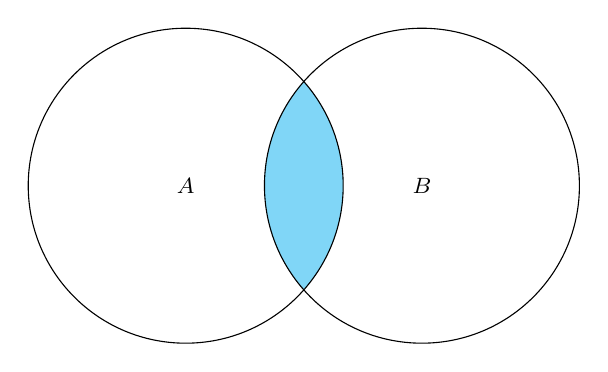
\begin{tikzpicture}[scale=1, font=\footnotesize, line join=round, line cap=round,>=stealth]
\coordinate (A) at (0,0);
\coordinate (B) at (3,0);
\begin{scope}
\clip(A) circle(2 cm);
\fill[cyan!50] (B) circle(2 cm);
\end{scope}
\draw (A) circle(2 cm) (B) circle(2 cm) (A)node{$A$} (B)node{$B$};
\end{tikzpicture}
\end{center}
Gọi $A, B$ lần lượt là tập hợp các học sinh giỏi và hạnh kiểm tốt của lớp $10\mathrm{A}$.\\
$\Rightarrow n(A)=12; n(B)=30; n(A\cap B)=10$.\\
Số học sinh được khen thưởng là \\
$n(A \cup B)=n(A)+n(B)-n(A\cap B)=12+30-10=32$.\\
Số học sinh không được khen thưởng là $45-32=13$ (học sinh).
}
\end{ex}

\begin{ex}%[0D4B4-4]
Cặp số $(x;y)=(-1;3)$ là nghiệm của hệ bất phương trình nào trong các hệ bất phương trình sau?
\def\dotEX{}
\choice
{$\heva{& x-y\le 2\\& 3x+2y\ge 2\\& y\le 0\\& x<0}$}
{$\heva{& x-y\le 2\\& 3x+y\ge 2\\& y\le 0\\& x<0}$}
{$\heva{& x-y\le 2\\& 3x+y\ge 2\\& y\ge 0\\& x<0}$}
{\True $\heva{& x-y\le 2\\& 3x+2y\ge 2\\& y\ge 0\\& x<0}
$}
\loigiai{Thay cặp số $(-1;3)$ vào hệ bất phương trình $\heva{& x-y\le 2\\& 3x+2y\ge 2\\& y\ge 0\\& x<0}$, ta có
$\heva{& -1-3 =-4 \le 2\\& 3 \cdot (-1)+2 \cdot 3 = 3 \ge 2\\& 3 \ge 0\\& -1<0}$ (đúng).
}
\end{ex}

\begin{ex}%[Trần Quốc, BG10-2022, Nhóm 9]%[0H1Y3-1]
Cho hai vectơ $\overrightarrow{a}$, $\overrightarrow{b}$ khác $\overrightarrow{0}$ thỏa mãn $\overrightarrow{a}=-\dfrac{1}{2}\overrightarrow{b}$. Mệnh đề nào dưới đây đúng?
\choice
{$\left|\overrightarrow{a}\right|=-\dfrac{1}{2}\left|\overrightarrow{b}\right|$}
{$\overrightarrow{a}$ và $\overrightarrow{b}$ là hai vectơ đối nhau}
{$\overrightarrow{a}$ cùng hướng với $\overrightarrow{b}$}
{\True $\overrightarrow{a}$ ngược hướng với $\overrightarrow{b}$}
\loigiai{
Do $\overrightarrow{a}=-\dfrac{1}{2}\overrightarrow{b}$ và $-\dfrac{1}{2}<0$ nên $\overrightarrow{a}$ ngược hướng với $\overrightarrow{b}$.
}
\end{ex}

\begin{ex}%[Đoàn Minh Tân]%[0D4Y5-1]
Tìm tham số $m$ để tam thức $f(x)=3x^2-2mx+1$ dương tại $x=1$.
\choice
{\True $m<2$}
{$m>2$}
{$m>-2$}
{$m<4$}
\loigiai{
$f(x)=3x^2-2mx+1$ dương tại $x=1$ $\Leftrightarrow f(1)>0\Leftrightarrow 3-2m+1>0\Leftrightarrow m<2$.
}
\end{ex}

\begin{ex}%[Đoàn Minh Tân]%[0D4Y5-1]
Tam thức bậc hai nào dưới đây có bảng xét dấu như hình vẽ?
\begin{center}

\begin{tikzpicture}
\tkzTabInit[nocadre=false, lgt=1.5, espcl=1.5]
{$x$ /0.6,$f(x)$ /0.6}
{$-\infty$,$1$,$3$, $+\infty$}
\tkzTabLine{,-,0,+,0,-}
\end{tikzpicture}
\end{center}
\choice
{$f(x)=x^2-4x+3$}
{\True $f(x)=-2x^2+8x-6$}
{$f(x)=-x^2-4x-3$}
{$f(x)=3x^2+12x+9$}
\loigiai{
Từ bảng xét dấu, suy ra tam thức $f(x)=ax^2+bx+c$ có hệ số $a<0$ và có hai nghiệm $x_1=1$, $x_2=3$.\\
Do đó, ta loại hai phương án $f(x)=x^2-4x+3$ và $f(x)=3x^2+12x+9$.\\
Xét phương án $f(x)=-2x^2+8x-6$ có $\Delta =16>0$, hai nghiệm $x_1=1$, $x_2=3$ (thoả mãn bảng xét dấu).\\
Xét phương án $f(x)=-x^2-4x-3$ có $\Delta =4>0$, hai nghiệm $x_1=-3$, $x_2=-1$ (không thoả mãn bảng xét dấu).\\
Vậy $f(x)=-2x^2+8x-6$.
}
\end{ex}
\Closesolutionfile{ans}

\noindent{\bf\fontfamily{qag}\selectfont\color{violet}B. PHẦN TỰ LUẬN}
\begin{ex}[1,0 điểm]%[0D2Y3-1]
Vẽ đồ thị hàm số $y = x^2 - 4x + 3$.
\loigiai
{ Xét hàm số $y = x^2 - 4x + 3$ có đồ thị là parabol $\left(P\right)$.
\begin{itemize}
\item $\left(P\right)$ có tọa độ đỉnh là $I(2;-1)$ và trục đối xứng $x = 2$.

\item Đồ thị
\begin{center}
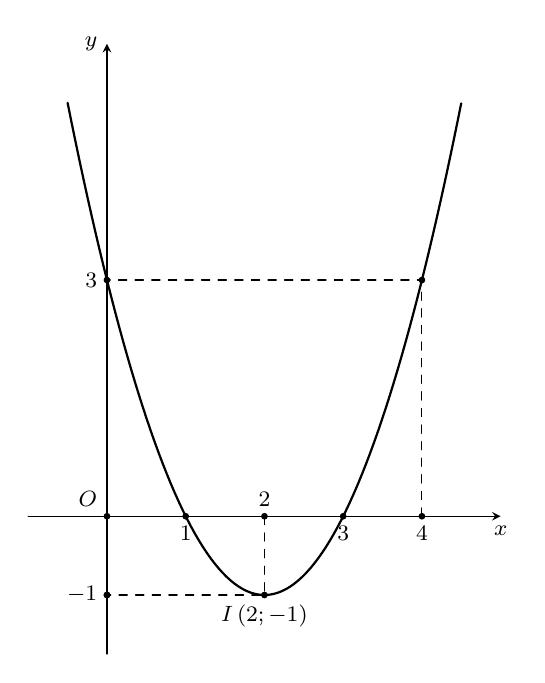
\begin{tikzpicture}[scale = 1, font=\footnotesize, line join=round, line cap=round, >=stealth]
\draw[->] (-1,0) -- (0,0) node[above left]{$O$} -- (5,0) node[below]{$x$};
\draw[->] (0,-1.75) -- (0,6) node[left]{$ y $};
\draw[color = black, thick] plot[domain=-0.5:4.5, samples=100](\x,{(\x)^(2)-4*(\x)+3});
\draw[fill=black] (1,0) node[below]{$ 1 $} circle (1pt);
\draw[fill=black] (3,0) node[below]{$ 3 $} circle (1pt);
\draw[fill=black] (4,0) node[below]{$ 4 $} circle (1pt);
\draw[fill=black] (0,3) node[left]{$ 3 $} circle (1pt);
\draw[fill=black] (0,-1) node[left]{$ -1 $} circle (1pt);
\draw[fill=black] (0,0) circle (1pt) (2,0)node[above]{$2$} circle (1pt) (2,-1) circle (1pt) (0,-1) circle (1pt) (4,3) circle (1pt);
\draw[dashed] (2,0)--(2,-1)node[below]{$I\left(2;-1\right)$}--(0,-1) (4,0)--(4,3)--(0,3);
\end{tikzpicture}
\end{center}
\end{itemize}
}
\end{ex}

\begin{ex}[0,5 điểm]%[Hoàng Thanh Phương, BG10-2022-Đợt 2, Nhóm 3]%[0D4B5-1]
Giải bất phương trình sau $x^2-7x+10\ge 0$ bằng cách lập bảng xét dấu.
\loigiai{
Tam thức bậc hai $f(x)=x^2-7x+10$ có $a=1>0$ và có hai nghiệm $x_1=2$, $x_2=5$. \\
Suy ra $x^2-7x+10\ge 0\Leftrightarrow \hoac{&x\le 2\\&x\ge 5.}$ \\
Vậy tập nghiệm của bất phương trình là $S=(-\infty;2]\cup [5;+\infty)$.
}
\end{ex}

\begin{ex}[0,5 điểm]%[Phan Anh]%[Dự án giáo án 10]%[0H1B2-5]
Cho hình chữ nhật $ABCD$ có $AC=5$, $AB=3$, xác định và tính độ dài của véc-tơ $\overrightarrow{b}=\overrightarrow{AB}+\overrightarrow{AC}$.
\loigiai{\begin{center}
\begin{tikzpicture}[>=stealth,line join=round,line cap=round,font=\footnotesize,scale=0.7]
\path (0,4) coordinate (A)
(3,4) coordinate (B)
(3,0) coordinate (C)
($(A)+(C)-(B)$) coordinate (D)
($(B)+(C)-(A)$) coordinate (E)
($(B)!0.5!(C)$) coordinate (M)
;
\draw (D)--(B)--(E)--(A)--(B)--(C)--(D)--(A)--(C);
\foreach\p /\r in {A/135,B/45,C/-45,D/-135,M/10,E/-45}
\fill (\p) circle (1.2pt) node[shift={(\r:3mm)}]{$\p$};
\end{tikzpicture}
\end{center}
Dựng $\overrightarrow{BE}=\overrightarrow{AC}$, ta có $\overrightarrow{b}=\overrightarrow{AB}+\overrightarrow{AC}=\overrightarrow{AB}+\overrightarrow{BE}=\overrightarrow{AE}$.\\
Suy ra $\left|\overrightarrow{b}\right|=\left|\overrightarrow{AE}\right|=AE$. Gọi $M$ là trung điểm của $BC$.\\
Ta có $AE=2AM=2\sqrt{AB^2+BM^2}=2\sqrt{13}$. Vậy $\left|\overrightarrow{b}\right|=2\sqrt{13}$.
}
\end{ex}

\begin{ex}[0,5 điểm]
Cho hai điểm $A$, $B$ cố định. Tìm tập hợp các điểm $M$ thoả $|\vec{MA}-3\vec{MB}|=2|\vec{MA}-\vec{MB}|$.
\end{ex}

\begin{ex}%[0T3K2-5]
    Một doanh nghiệp tư nhân A chuyên kinh doanh xe gắn máy các loại. Hiện nay doanh nghiệp đang tập trung chiến lược vào kinh doanh xe hon đa Future Fi với chi phí mua vào một chiếc là $27$ triệu đồng và bán ra với giá là $31$ triệu đồng. Với giá bán này thì số lượng xe mà khách hàng sẽ mua trong một năm là $600$ chiếc. Nhằm mục tiêu đẩy mạnh hơn nữa lượng tiêu thụ dòng xe đang ăn khách này, doanh nghiệp dự định giảm giá bán và ước tính rằng nếu giảm $1$ triệu đồng mỗi chiếc xe thì số lượng xe bán ra trong một năm là sẽ tăng thêm $200$ chiếc. Vậy doanh nghiệp phải định giá bán mới là bao nhiêu để sau khi đã thực hiện giảm giá, lợi nhuận thu được sẽ là cao nhất.
    % \dapso{$30{,}5$ triệu đồng.}
    \loigiai{
    }
\end{ex}